\documentclass[12pt]{report}
\usepackage{graphicx}
\usepackage{float}
\begin{document}

\paragraph{Project:} NanoLab Evaporator Source Feedthrough
\paragraph{Goal:} To create an electrical feedthrough for a joule heating-based evaporative source. It must hold two sources at the height of the window in the chamber. All the electrical paths must be able to carry 400W, and everything in the chamber must be stable in high vacuum. There must also be a shield to prevent the sources from depositing on each other. The entire system must drop out of the bottom of the evaporator to quickly replace the sources.

\paragraph{Engineering Work:}
In the first design, we used only one source which simplified the problem. We didn't need to worry about two feedthroughs and the interference between two sources. Here are the drawings for those parts. They are made of solid copper rod.

$$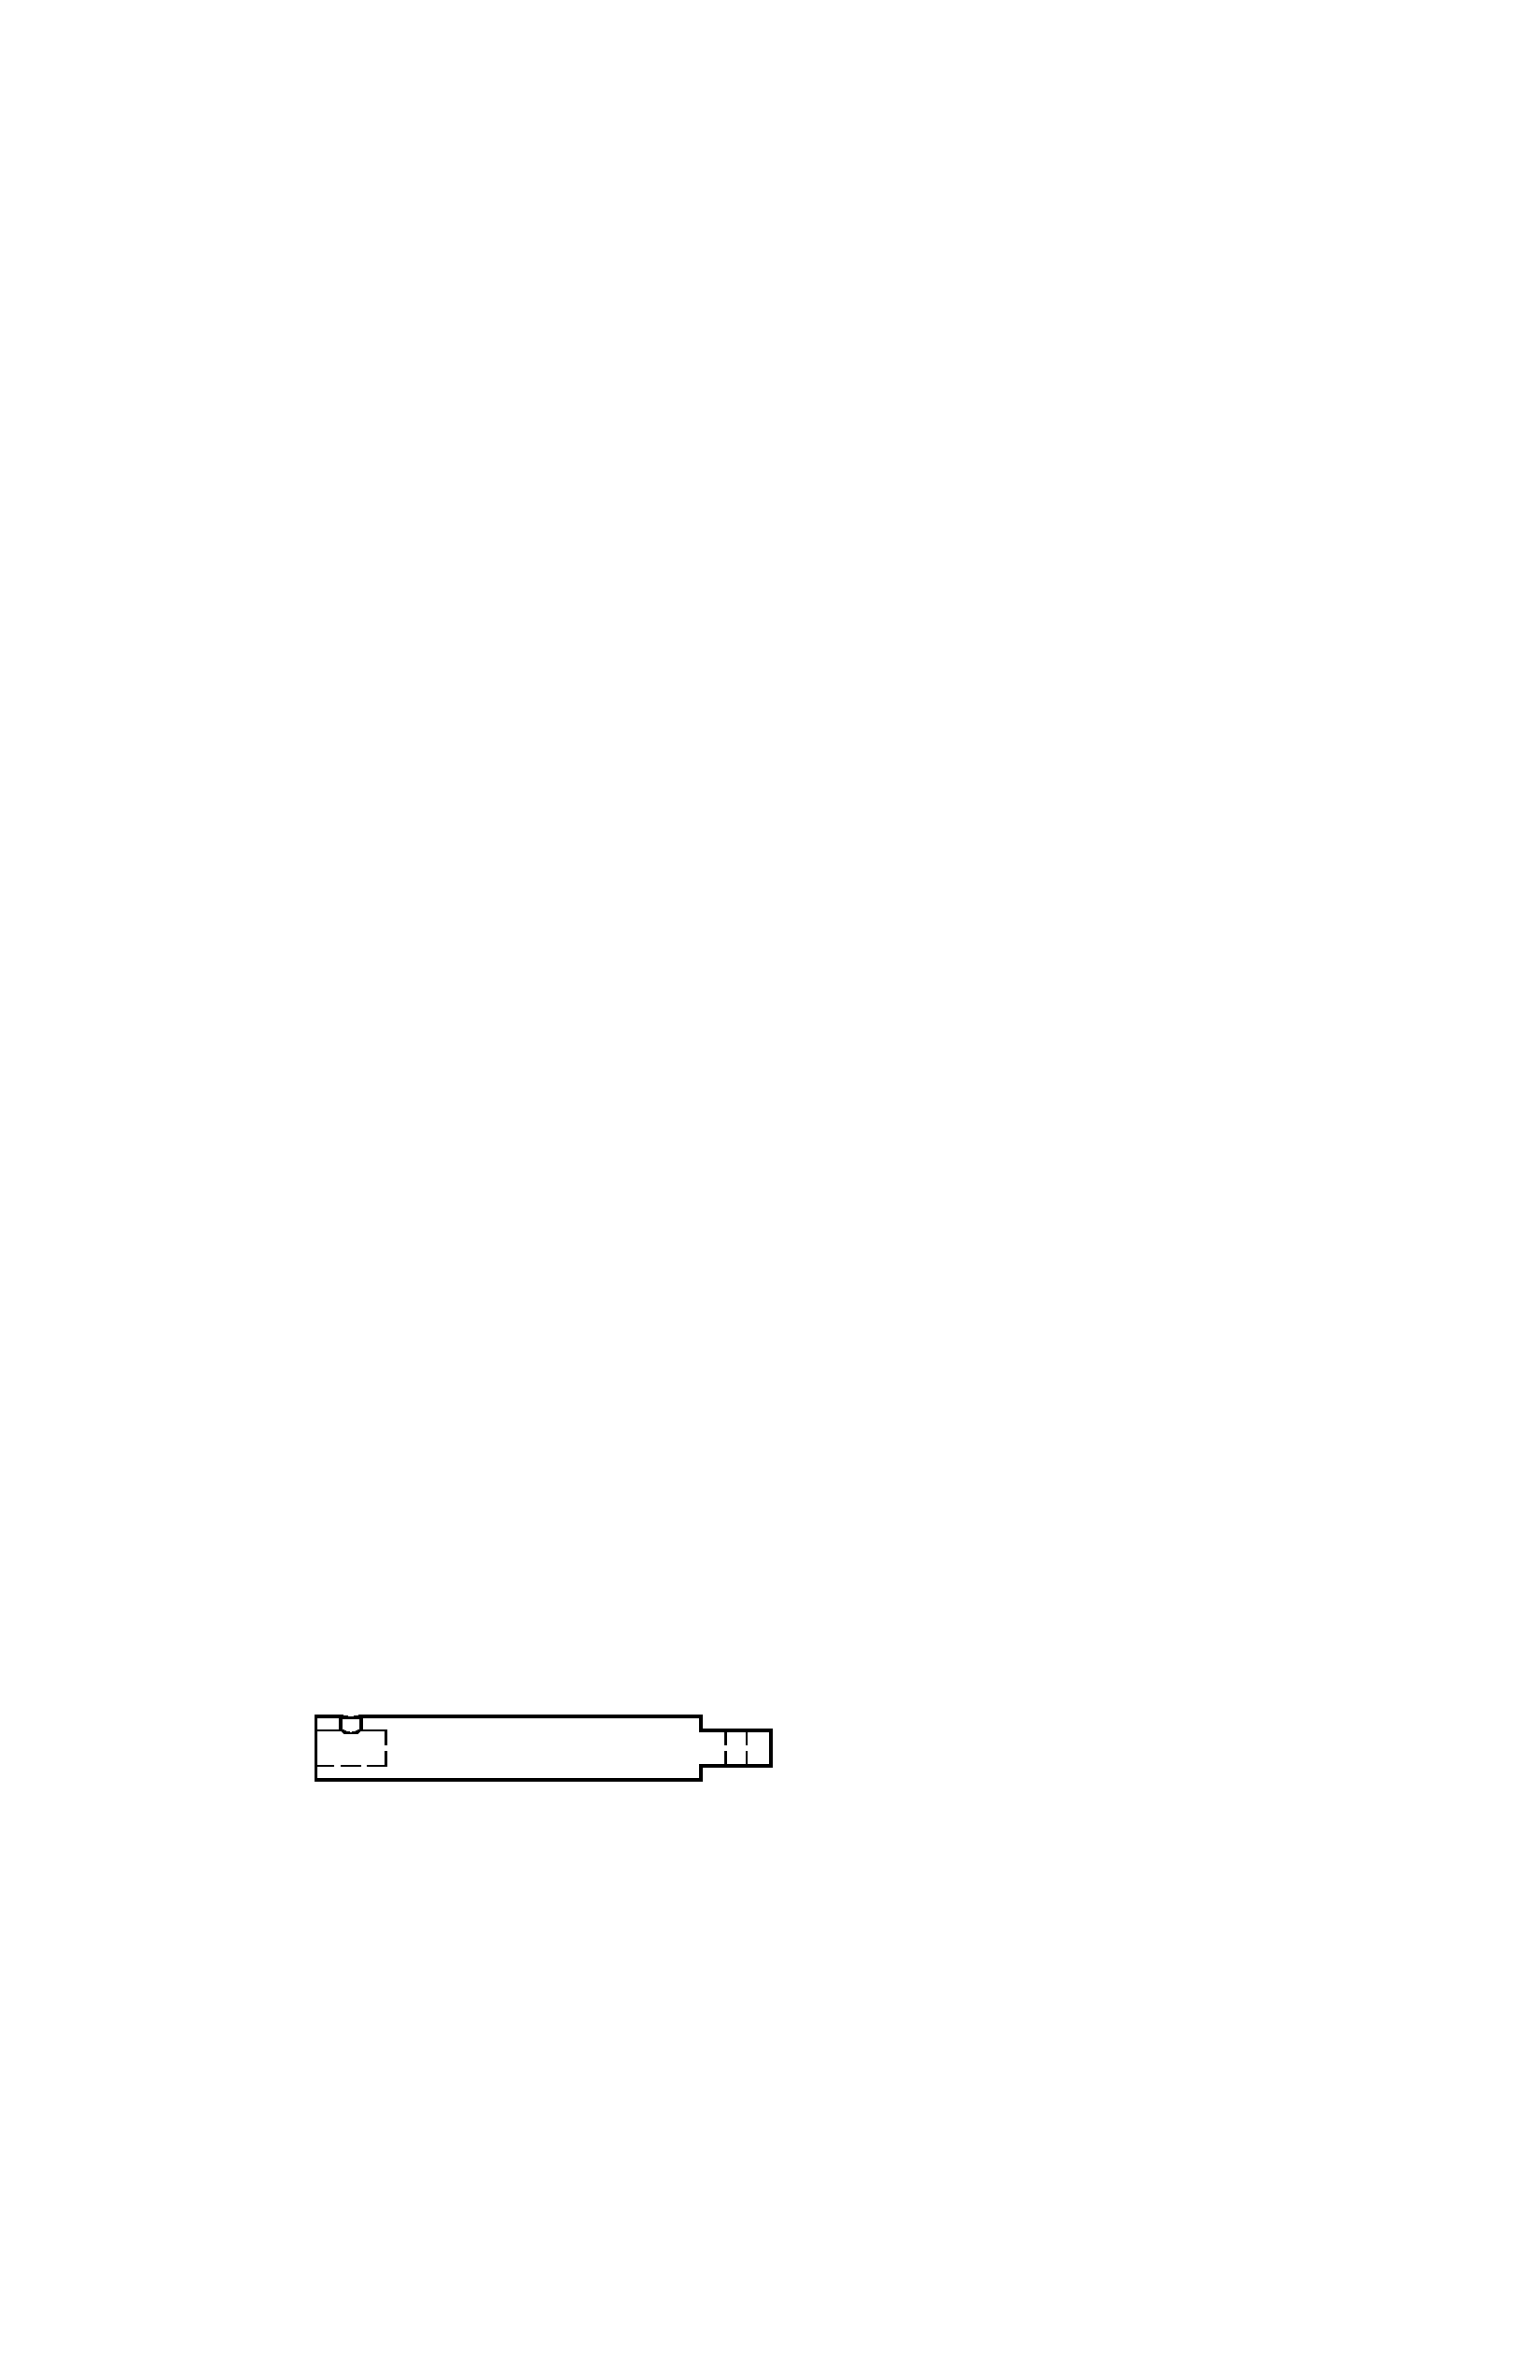
\includegraphics[scale=0.7]{fig1}$$
There are similar parts on the exterior that are shorter since they only need to adapt to some kind of attachment. This version had some issues - mainly with the way to hold the boats. The two posts were too close together and the boats often fell out of the holder. To change this, when we moved to the two source version, we tried to make the system wider. This means that the bottom of the evaporator must be larger to accommodate this. We changed the system so that the column is now a 3-inch adaptor from LF 160 to CF 8 and then a CF 8 to CF 2-3/4 zero length adaptor. The feedthrough then attaches to that plate. The whole plate will drop every time the sources need changing. \\
This gives us a 6 inch diameter clearance for the sources. The new system has arms that clamp onto the feedthrough and split out. This lets the two posts be further apart. 
$$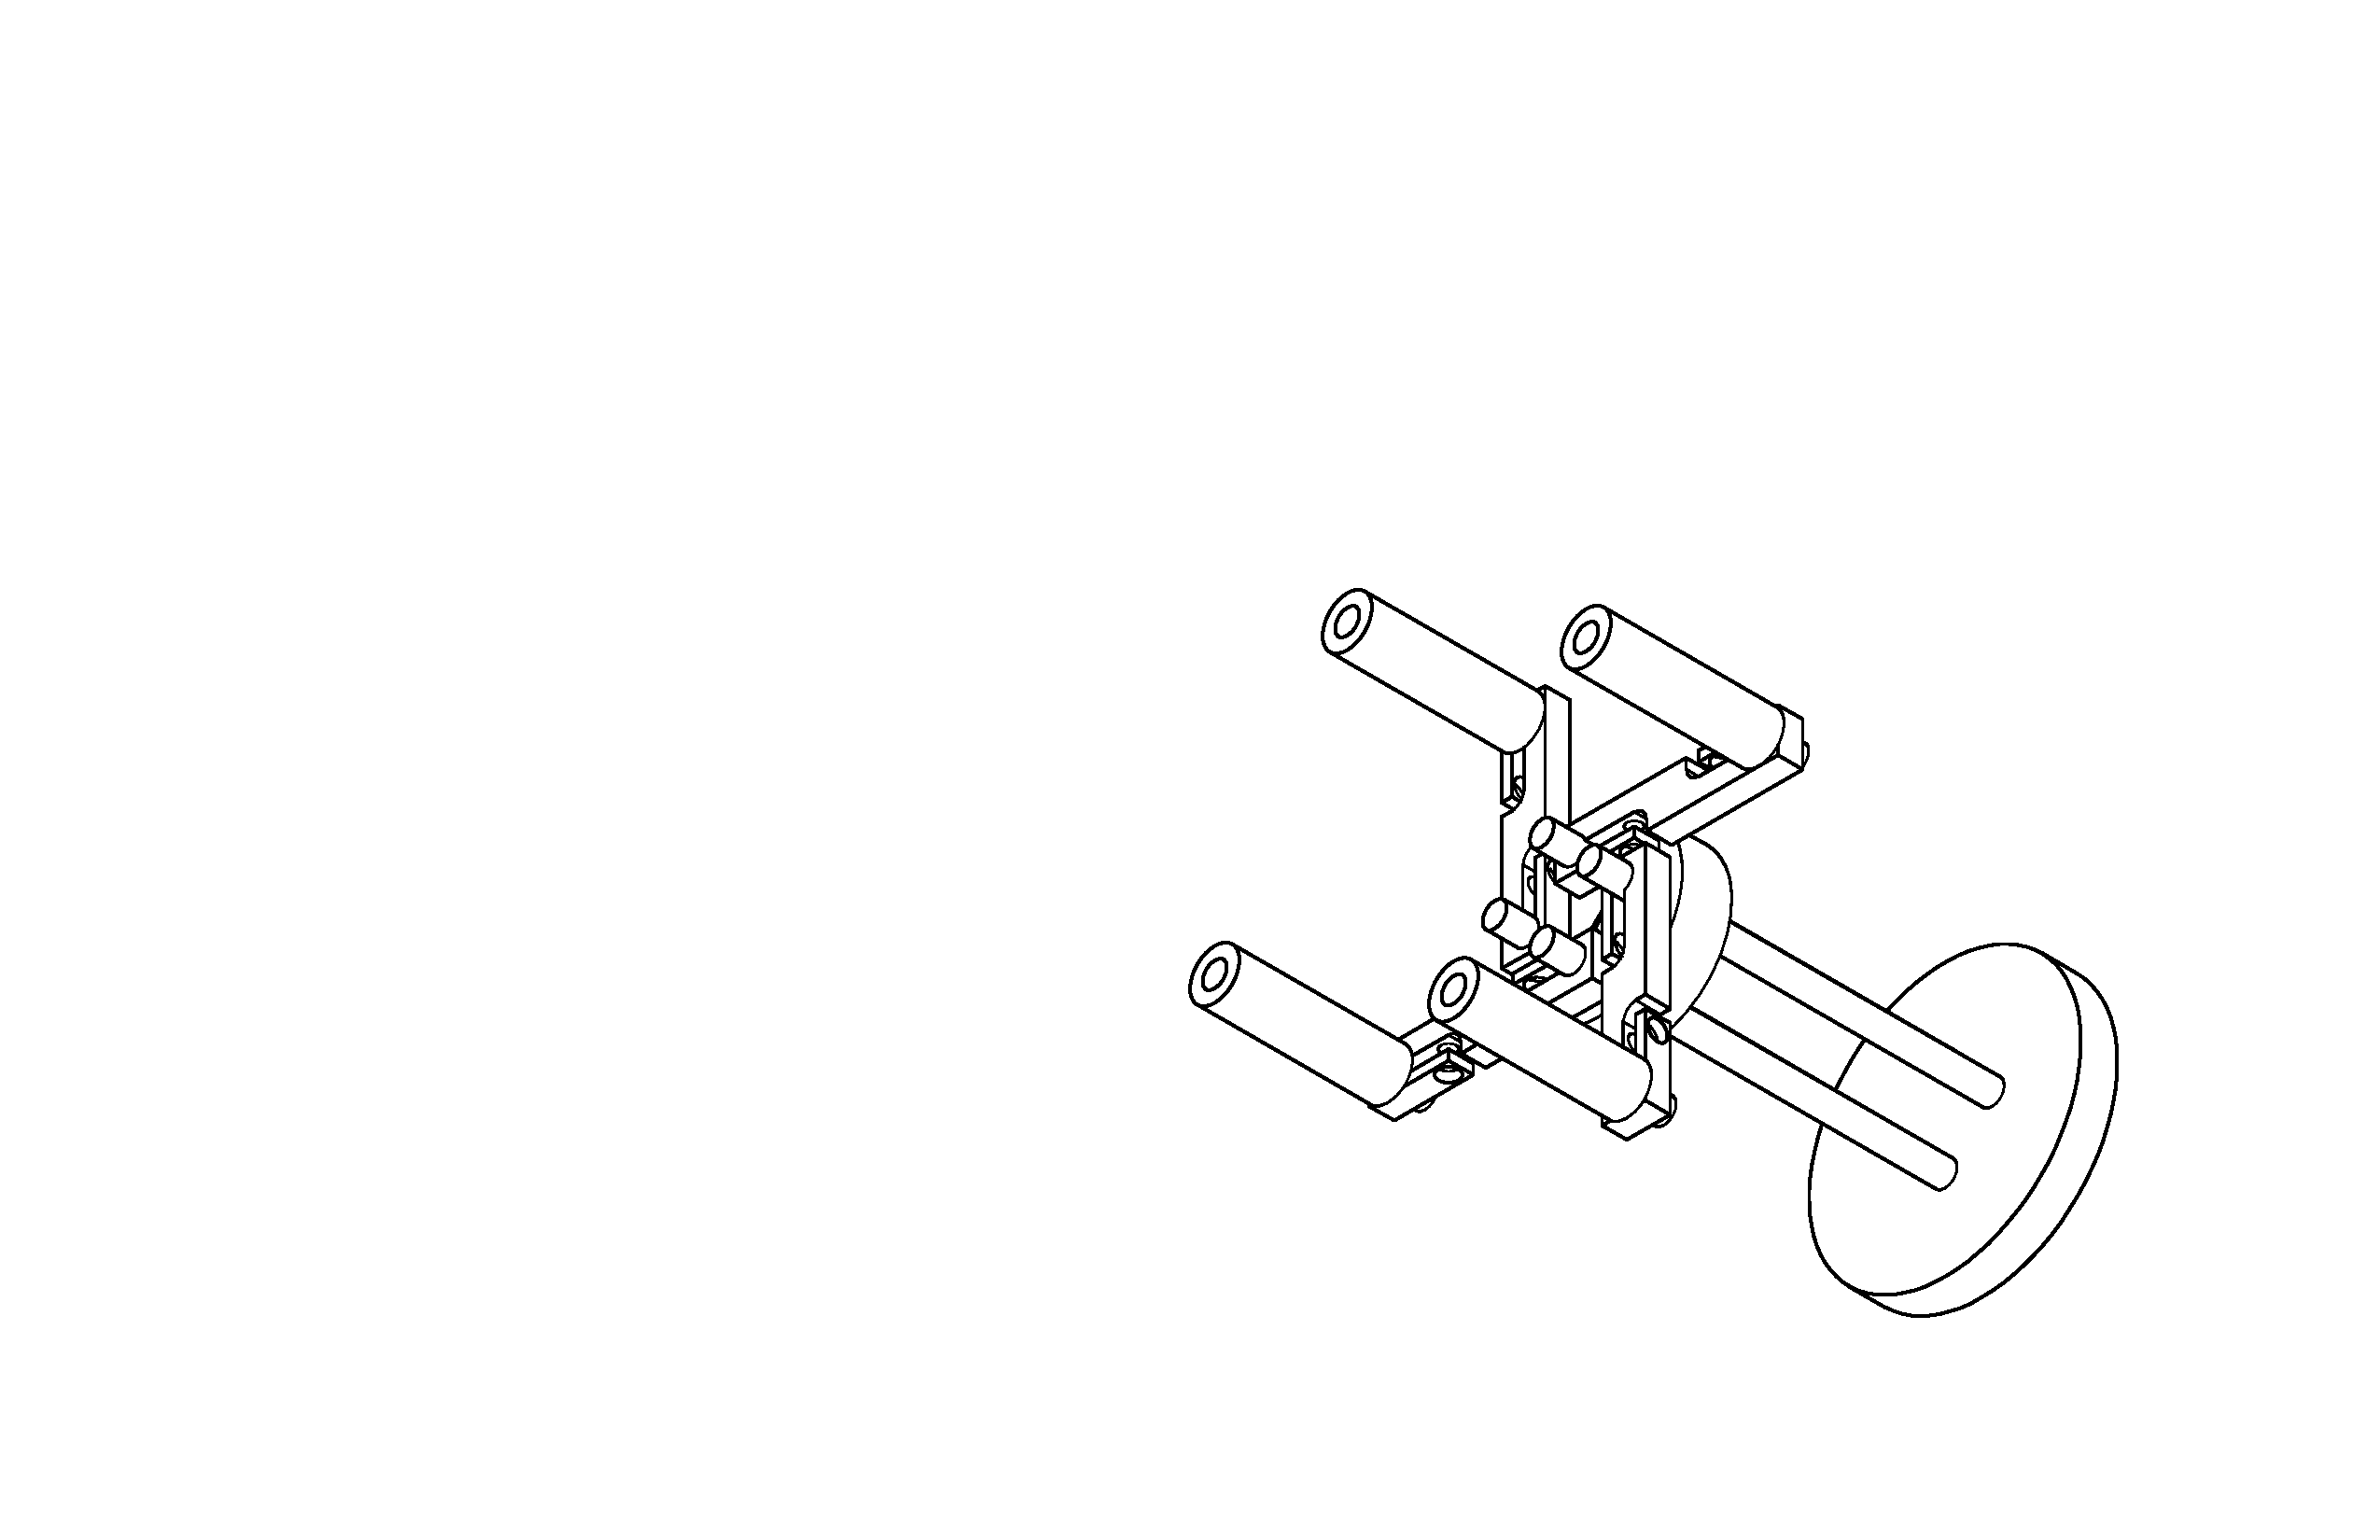
\includegraphics[scale=0.7]{fig2}$$
There are three components in this piece other than the feedthrough. The first is the post extension - this is just a tapped hole on one end for a screw to pinch the boat and a 1/4" nub on the other to be grabbed by the arm. The arm is more complicated. It has two holes to grab onto the feedthrough and the post, and then holes in the side for screws to tighten down on these two rods.
$$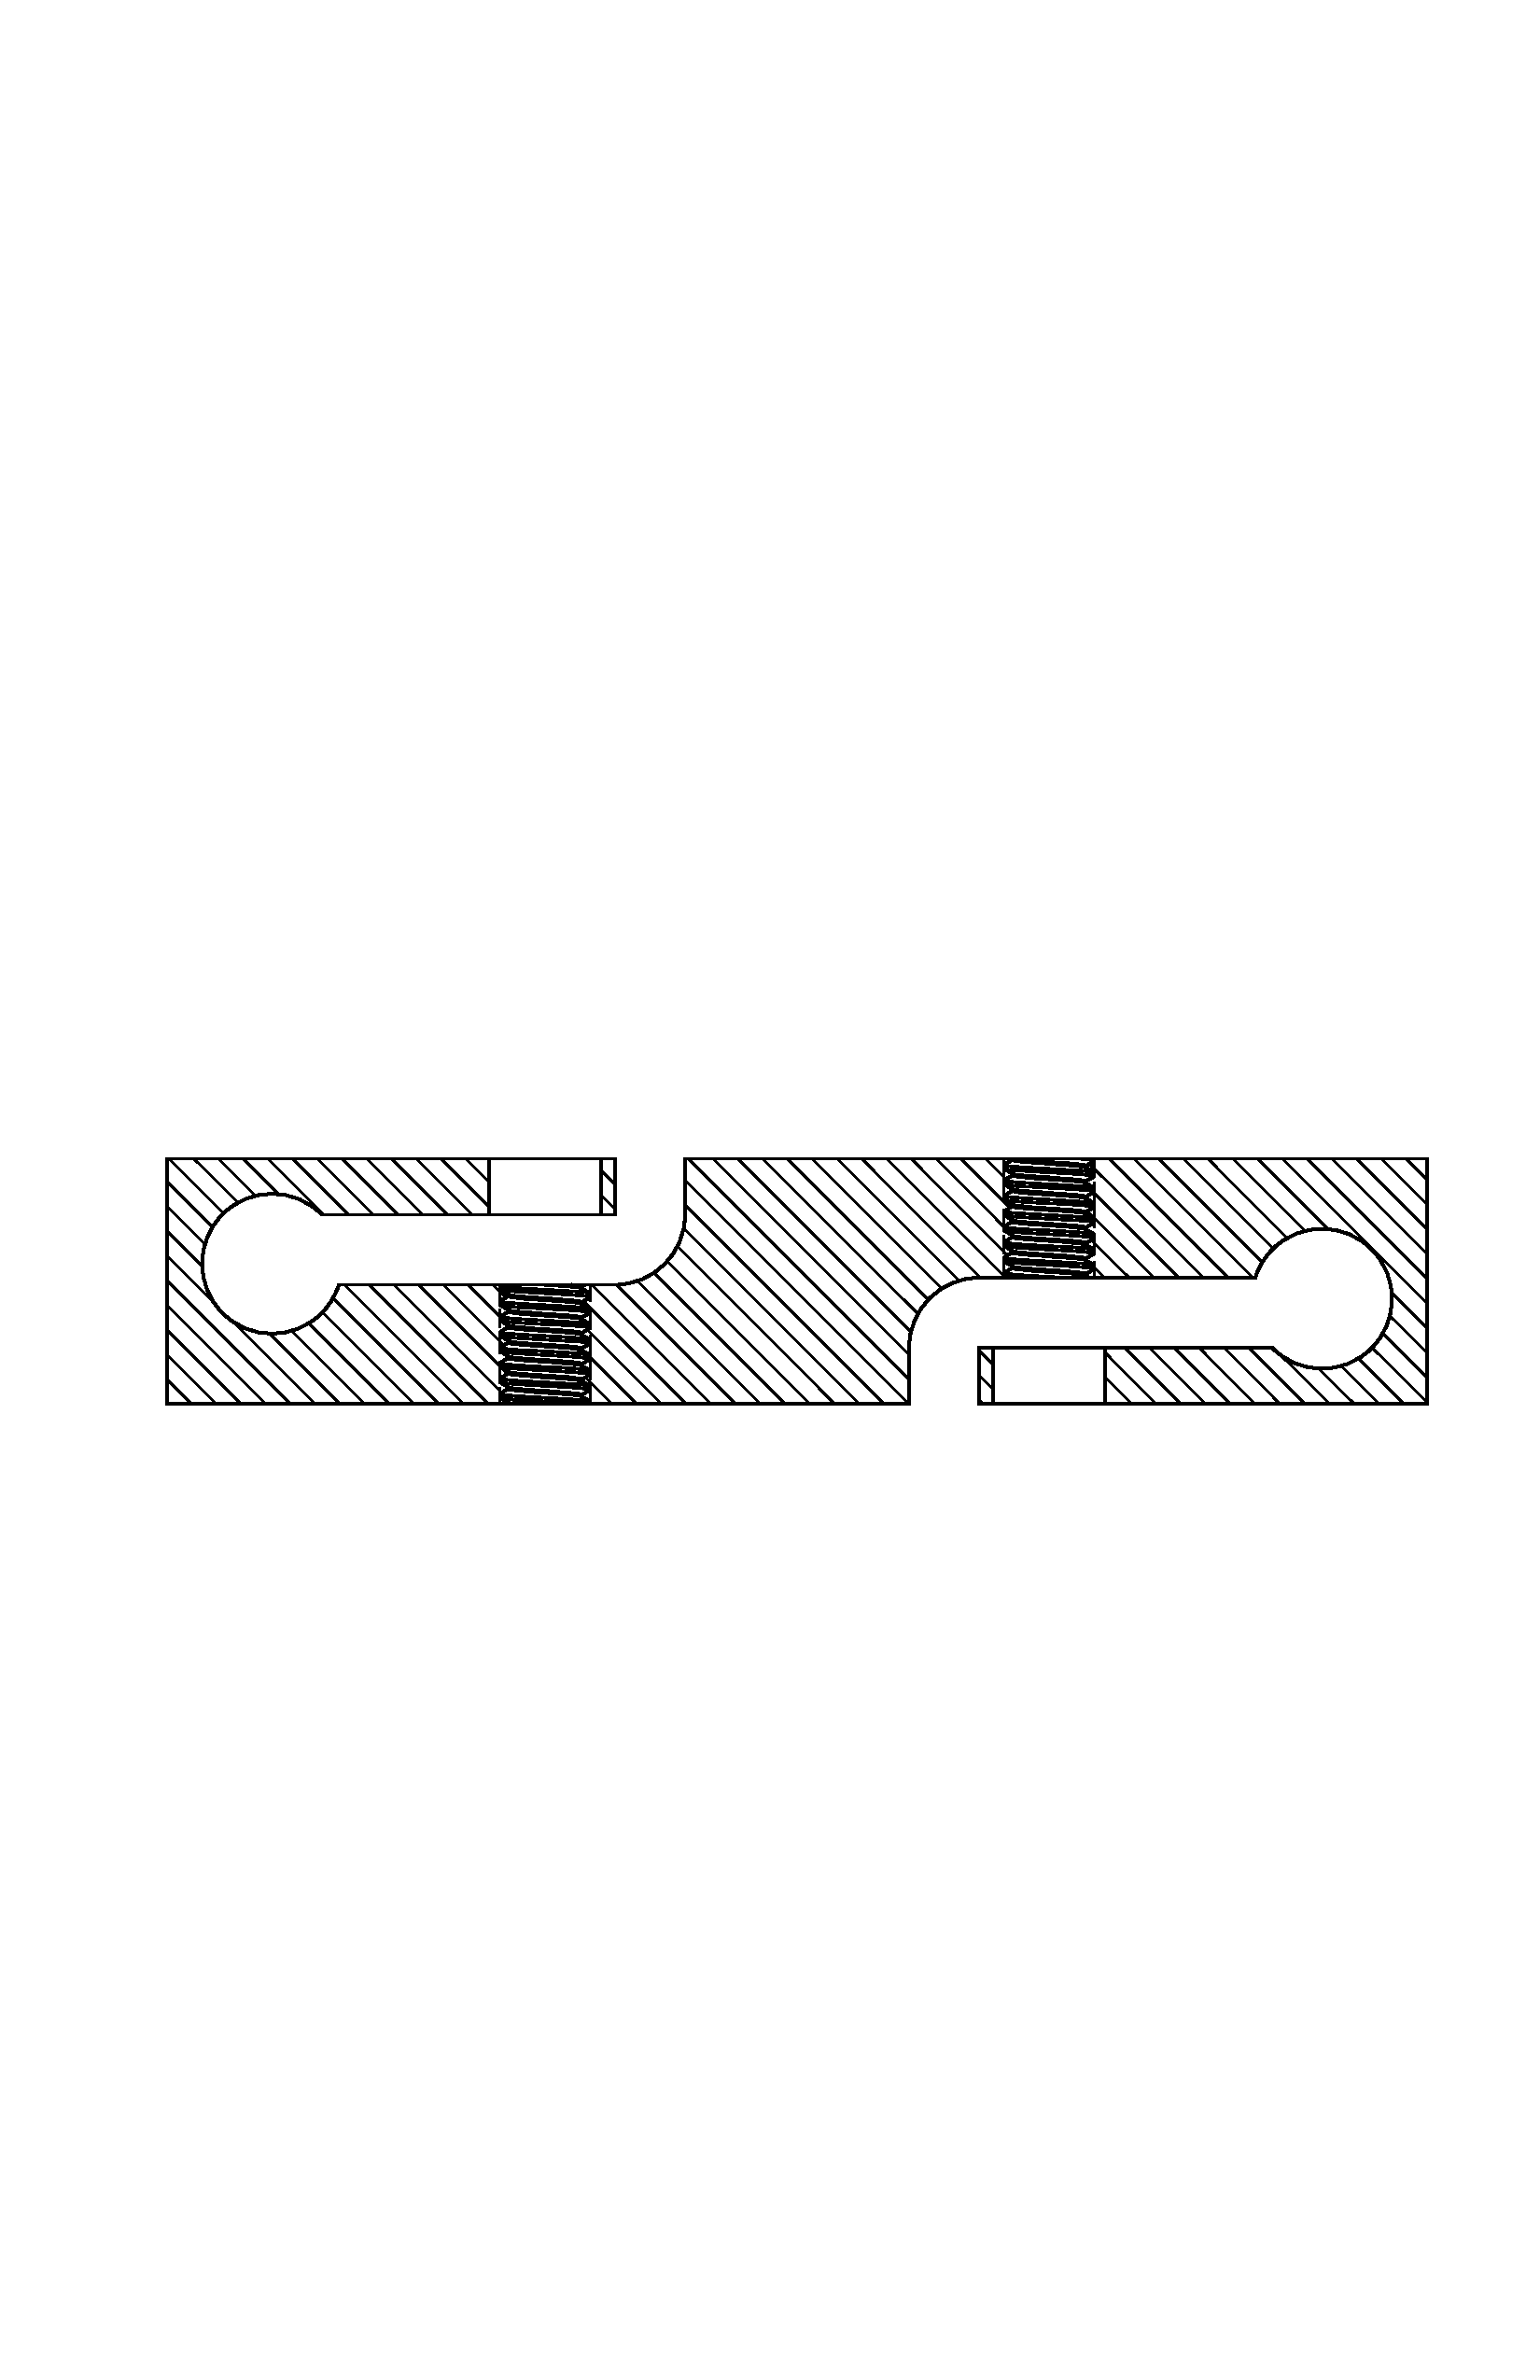
\includegraphics[scale=0.5]{fig3}$$
The copper is very flexible, so the smallest change in the diameter of the hole can dramatically affect how far the arm bends while tightening. The last piece is the Teflon washer. It pushes the four posts apart and holds a metal sheet to prevent the sources from depositing on each other. There is a small cut down the center of it to hold the sheet in place. The details of this have not been completely worked out. We have yet to machine any components for the outside, but they will probably have the same mating style as the arms inside and then some way to attach wires to that. 
\paragraph{Machining}
The posts are simple lathe pieces - drill a hole into one end at least 1/2" deep and then tap to 1/4-20. Extend the piece out of the collet by 8" and then part it off. Turn it around and reduce the diameter to 1/4" for about the bottom 3/8" of the part.\\
The arms are done entirely on the mill. Rough out the dimensions from stock - our stock was too large so I cut it down on the bandsaws. First I drilled and tapped the holes in the side. Then I used strap clamps to attach it to the table to drill the 1/4" holes and mill out the relief with CNC.

\paragraph{Source Changing Procedure}
As it currently stands, a person changing the source needs to unscrew all of the bolts on the CF 8 flange, then lower the massive plate without damaging the electrical feedthrough sticking out of the bottom, which has proven easy to bend. Then change out the baskets, put in the pellets, and raise it again. This is going to be very annoying and difficult. We need to design some system to raise and lower the feedthrough system safely. It would also be good if it could slide out from under the evaporator to make changing baskets easier.

\paragraph{Components List:} \hspace{1cm} \\
\begin{tabular}{c|c|c}
Part & Number/Requirements & Supplier\\
\hline
Electrical Feedthrough & FTT0543253 & Lesker \\
Copper Rod & 1/2" Diameter, 3ft & -\\
Copper Bar & 1/2" x 3/8" x 1ft & -\\
Teflon Disk & 3" Diameter, 1/2" & -\\ 
Asstd. Stainless Hardware & 1/4-20, M4 x 10mm& - 

\end{tabular}


\end{document}